\section{Bibliography}
\begin{thebibliography}{widestlabel}
	\bibitem{unityLessons}
	unitylessons.com. 2014. \textit{Unity3D Tutorial - Pickup and Carry Objects}.
	\newline
	[Online]. [Accessed 16 December 2015].\\
	Available from: \url{https://youtu.be/runW-mf1UH0}
	
	\bibitem{portalGame}
	\textit{Portal} (standard edition). 2007.\\
	PC / Mac, Playstation® 3, Xbox 360 [Game].\\
	Valve: Bellevue, Washington.
	
	\bibitem{portalChamberPic}
	Klow. 2009. \textit{Testchmb03.jpg}. [Online].
	\newline
	[Accessed 17 December 2015].\\
	Available from: \url{http://half-life.wikia.com/wiki/File:Testchmb03.jpg}
\end{thebibliography}

\pagebreak
\section{Appendix}
\subsection{Project files}
\begin{figure}[h!]
	\centering
	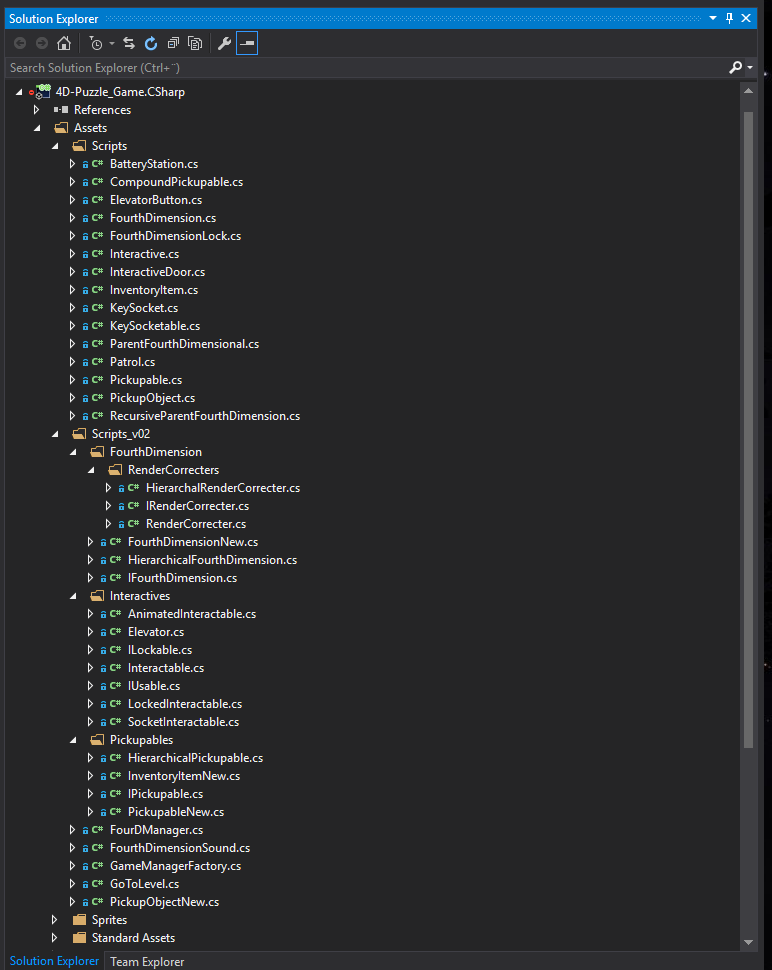
\includegraphics[scale=0.7]{pictures/FileOverview.png}
	\caption{All project files created throughout the course.}
	\label{projectFiles}
\end{figure}

\pagebreak
\subsection{Figures}
\begin{figure}[h!]
	\centering
	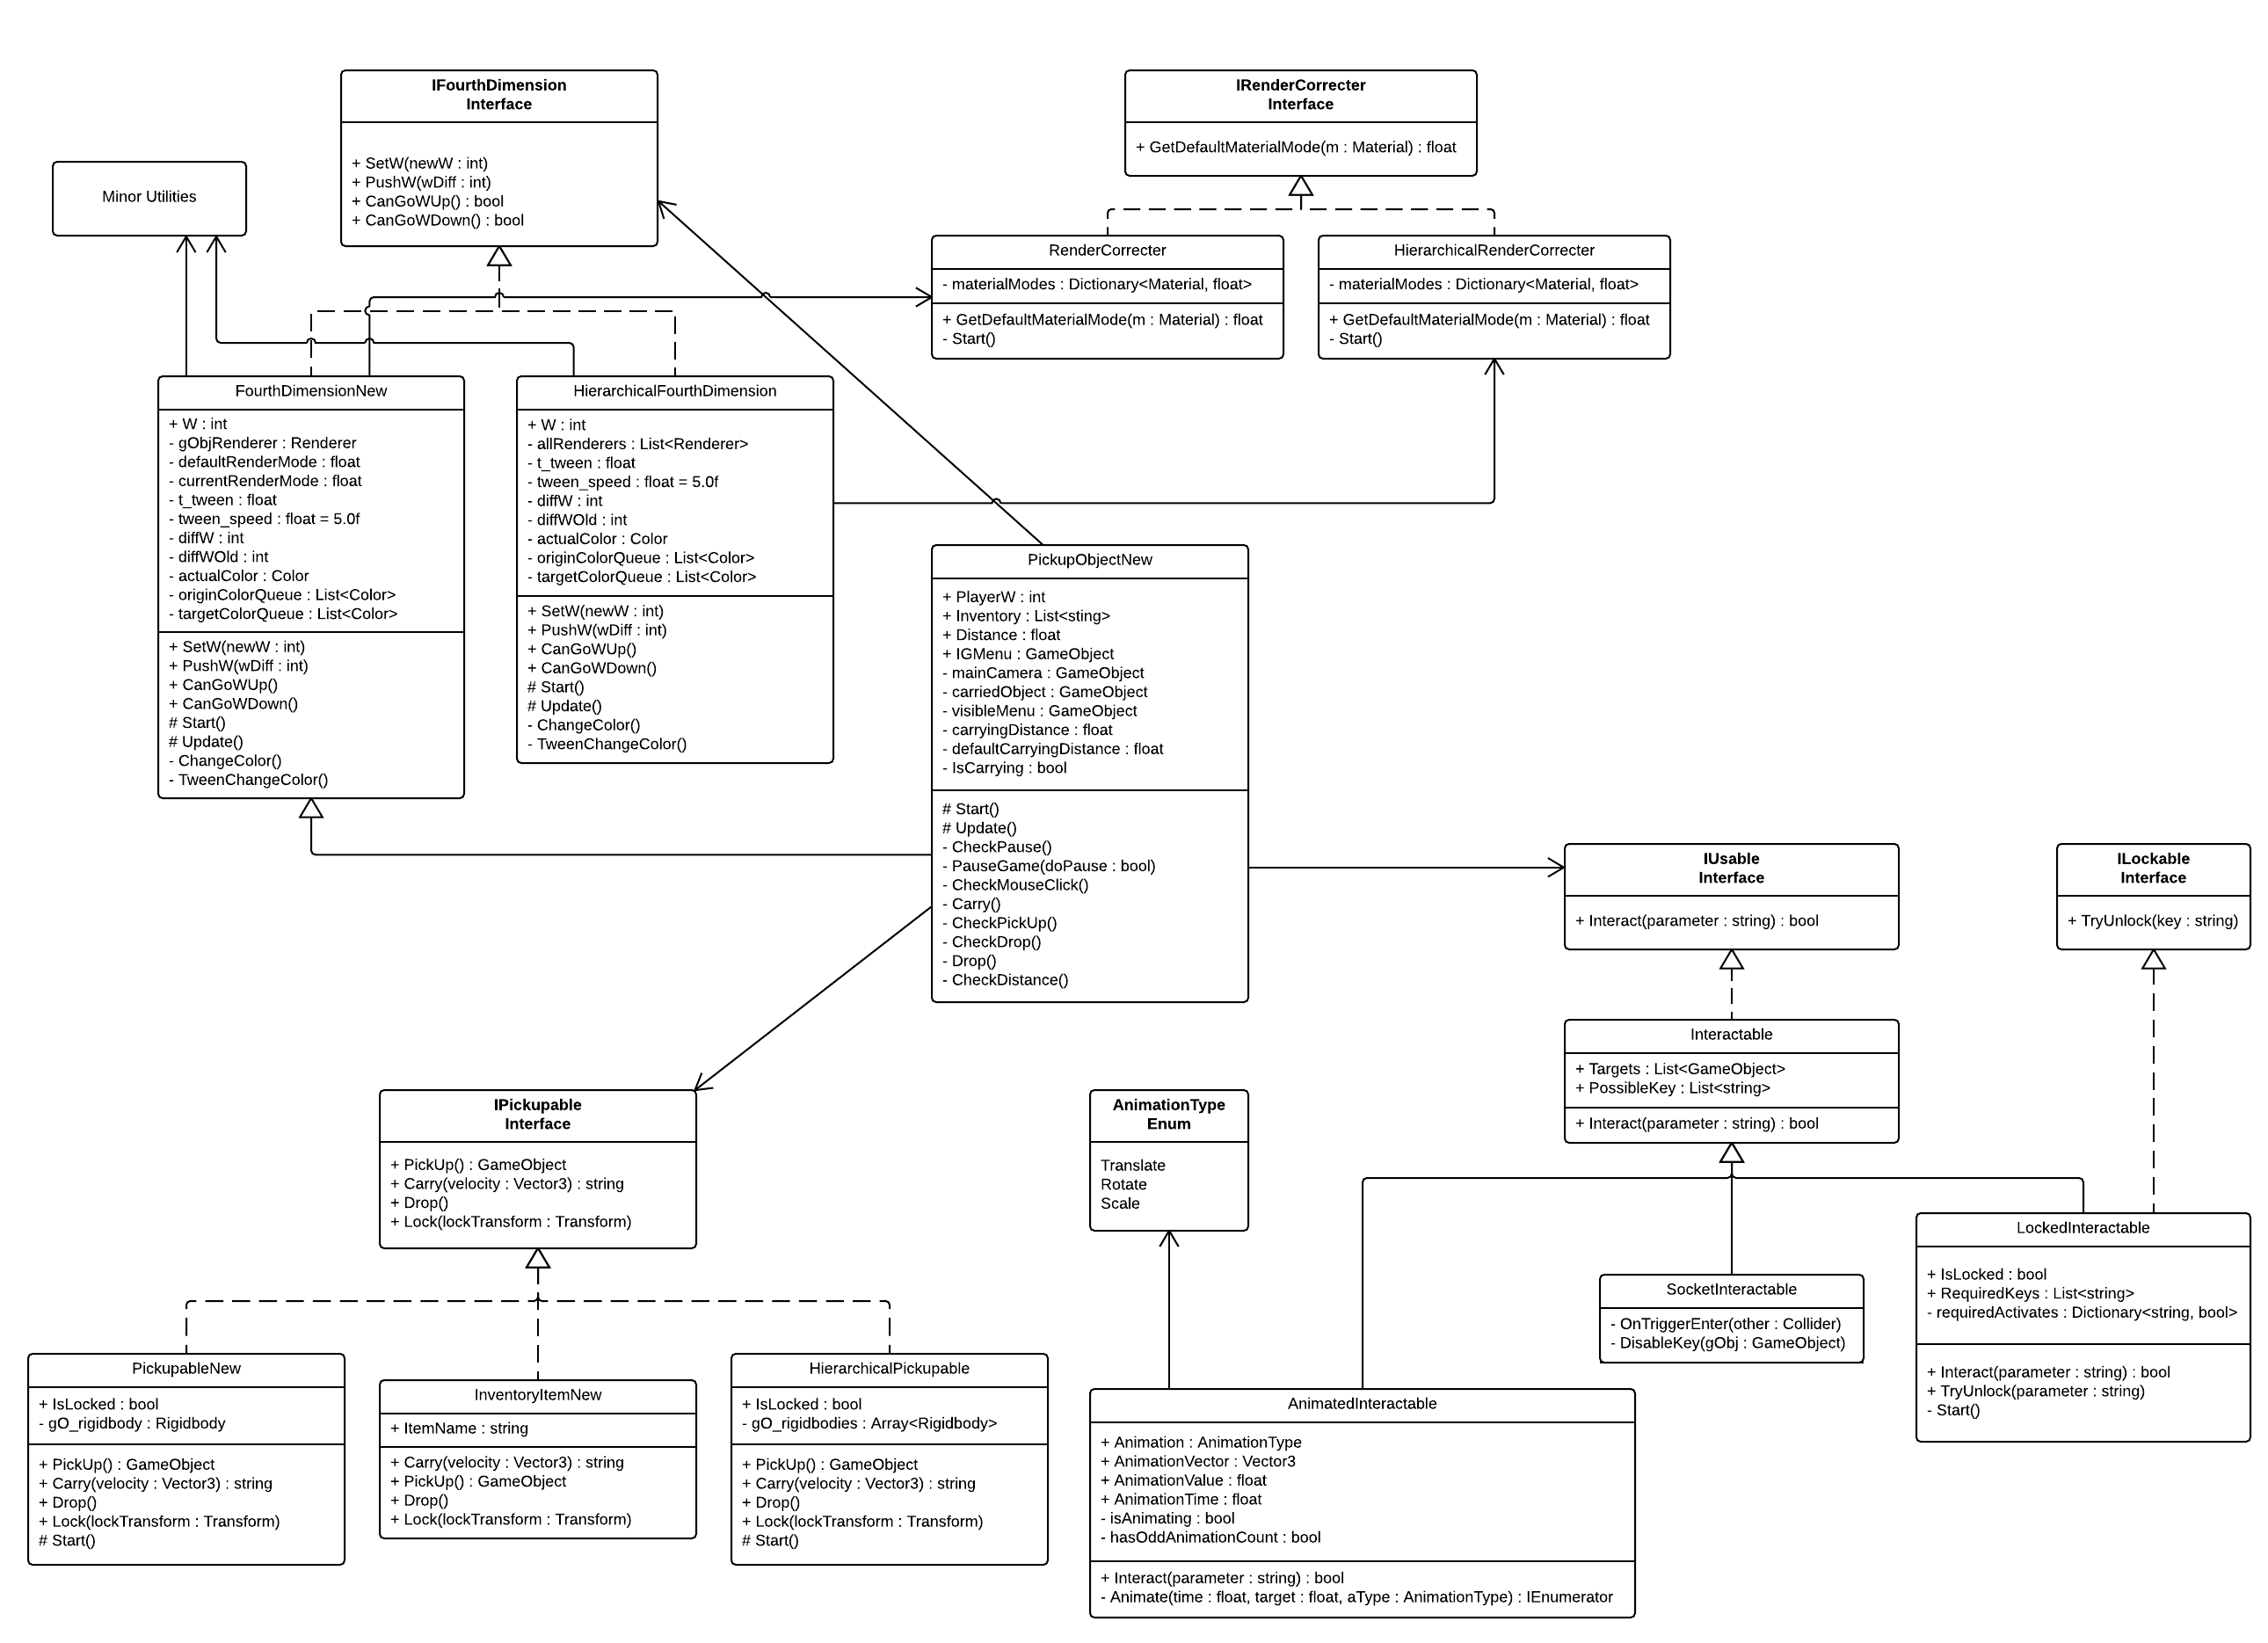
\includegraphics[angle=90,origin=c,scale=0.5]{pictures/4D-Puzzle-Flowchart.png}
	\caption{The entirety of our system architecture, expressed in UML}
	\label{completeUML}
\end{figure}

\begin{figure}[h!]
	\centering
	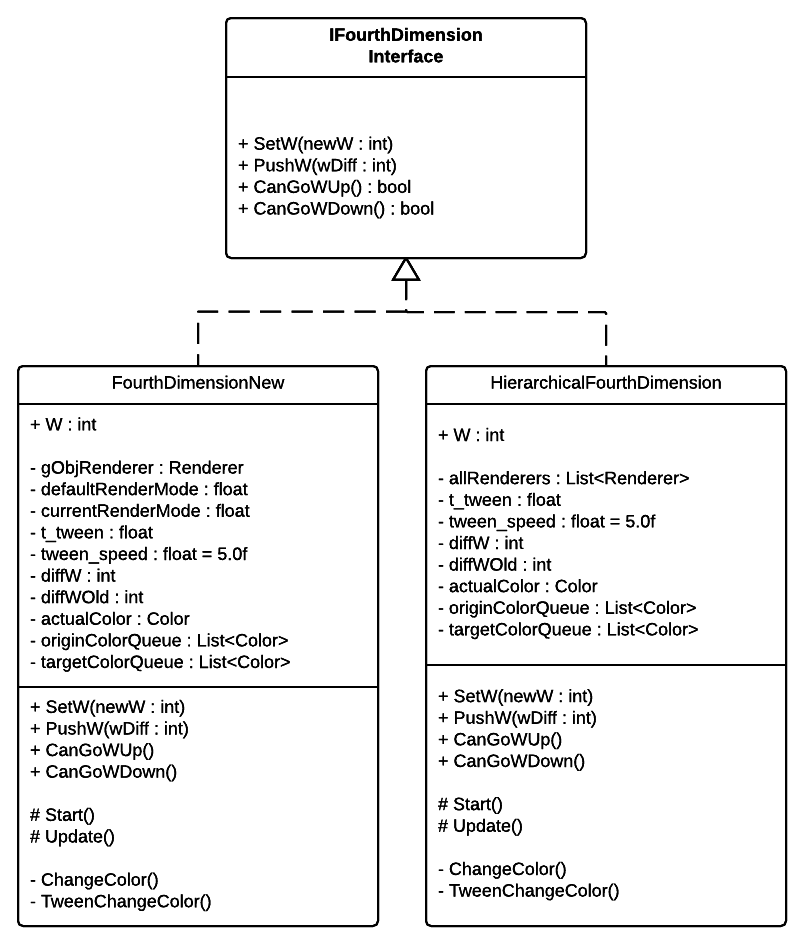
\includegraphics[scale=1]{pictures/FourthDimensionUML.png}
	\caption{The FourthDimension architecture, expressed in UML}
	\label{fourthOnlyUML}
\end{figure}

\begin{figure}[h!]
	\centering
	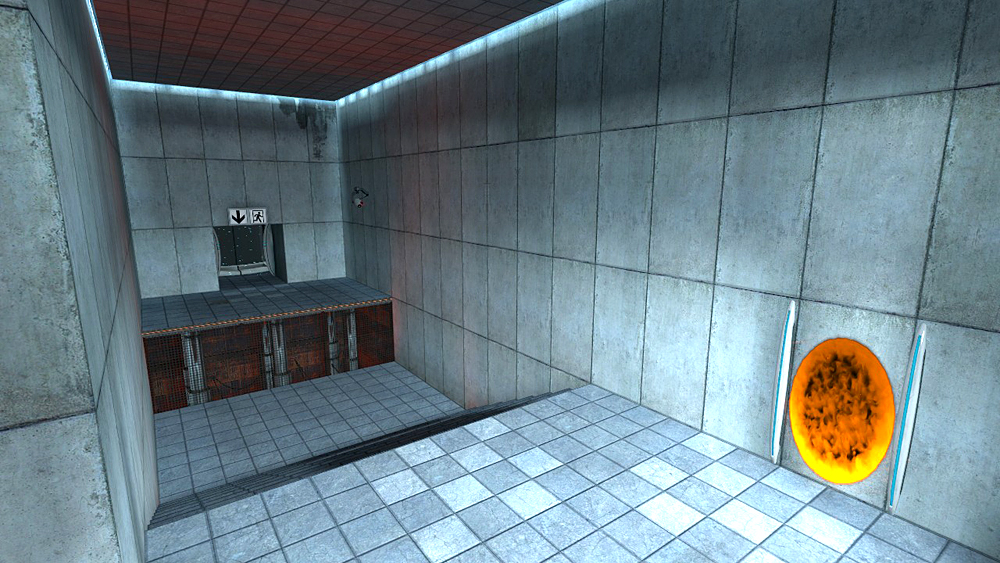
\includegraphics[angle=90,origin=c,scale=0.6]{pictures/portalChamber.jpg}
	\caption{A test chamber, as seen in Portal.\cite{portalChamberPic}}
	\label{portalChamber}
\end{figure}
